% ---- pg-052 （书页 40） ----

\begin{mvfigure}
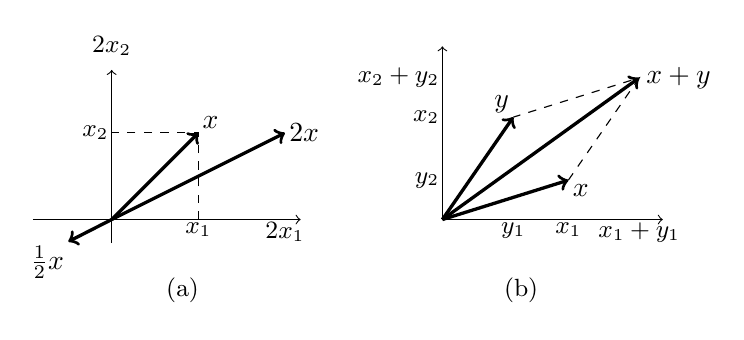
\begin{tikzpicture}[scale=1.0]
\begin{scope}[shift={(0,0)}]
\draw[->] (-1.0,0) -- (2.4,0);
\draw[->] (0,-0.3) -- (0,1.9);
\draw[dashed] (1.1,0) -- (1.1,1.1) -- (0,1.1);
\draw[very thick,->] (0,0) -- (1.1,1.1) node[above right,inner sep=1pt] {$\bm{x}$};
\draw[very thick,->] (0,0) -- (2.2,1.1) node[right,inner sep=1pt] {$2\bm{x}$};
\draw[very thick,->] (0,0) -- (-0.55,-0.28) node[below left,inner sep=1pt] {$\frac{1}{2}\bm{x}$};
\draw (0,1.1) node[left,inner sep=1pt] {\small $x_2$};
\draw (1.1,0) node[below,inner sep=1pt] {\small $x_1$};
\draw (2.2,0) node[below,inner sep=1pt] {\small $2x_1$};
\draw (0,2.2) node {\small $2x_2$};
\draw (0.9,-0.9) node {\small (a)};
\end{scope}
\begin{scope}[shift={(4.2,0)}]
\draw[->] (0,0) -- (2.8,0);
\draw[->] (0,0) -- (0,2.2);
\draw[very thick,->] (0,0) -- (1.6,0.5) node[below right,inner sep=1pt] {$\bm{x}$};
\draw[very thick,->] (0,0) -- (0.9,1.3) node[above left,inner sep=1pt] {$\bm{y}$};
\draw[dashed] (1.6,0.5) -- (2.5,1.8) -- (0.9,1.3);
\draw[very thick,->] (0,0) -- (2.5,1.8) node[right,inner sep=2pt] {$\bm{x}+\bm{y}$};
\draw (0,0.5) node[left,inner sep=1pt] {\small $y_2$};
\draw (0,1.3) node[left,inner sep=1pt] {\small $x_2$};
\draw (0,1.8) node[left,inner sep=1pt] {\small $x_2+y_2$};
\draw (1.6,0) node[below,inner sep=1pt] {\small $x_1$};
\draw (0.9,0) node[below,inner sep=1pt] {\small $y_1$};
\draw (2.5,0) node[below,inner sep=1pt] {\small $x_1+y_1$};
\draw (1.0,-0.9) node {\small (b)};
\end{scope}
\end{tikzpicture}
\phantomsection\label{fig:2.2}\mvcap{图 2.2\quad 标量乘法与向量加法}
\end{mvfigure}

\[
\bm{x}+\bm{y}=\begin{bmatrix}x_1\\x_2\\\vdots\\x_n\end{bmatrix}+\begin{bmatrix}y_1\\y_2\\\vdots\\y_n\end{bmatrix}=\begin{bmatrix}x_1+y_1\\x_2+y_2\\\vdots\\x_n+y_n\end{bmatrix}
\]

因此,$\bm{x}+\bm{y}$ 是一个向量,其第 $i$ 个元素为 $x_i+y_i$.

两个从坐标原点出发的向量之和,是以这两个向量为邻边所构成的平行四边形的对角
线,其几何解释见\hyperref[fig:2.2]{图 2.2}(b).

一个向量既有方向又有长度. 考虑 $n=2$ 维情形下的向量

\[
\bm{x}=\begin{bmatrix}x_1\\x_2\end{bmatrix}
\]

$\bm{x}$ 的长度记做 $L_x$,其定义为

\[
L_x=\sqrt{x_1^2+x_2^2}
\]

一个二维向量的长度在几何上可视做直角三角形斜边的长度,如\hyperref[fig:2.3]{图 2.3} 所示.

\begin{mvfigure}
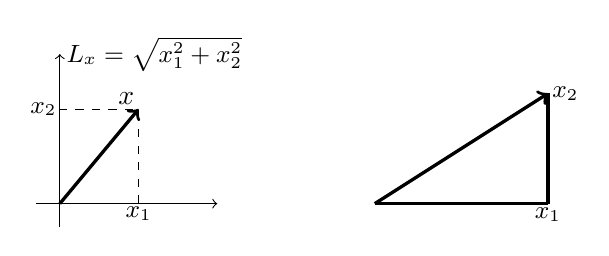
\begin{tikzpicture}[scale=1.0]
\begin{scope}[shift={(0,0)}]
\draw[->] (-0.3,0) -- (2.0,0);
\draw[->] (0,-0.3) -- (0,1.9);
\draw[dashed] (1.0,0) -- (1.0,1.2) -- (0,1.2);
\draw[very thick,->] (0,0) -- (1.0,1.2) node[above left,inner sep=1pt] {$\bm{x}$};
\draw (0,1.2) node[left,inner sep=1pt] {\small $x_2$};
\draw (1.0,0) node[below,inner sep=1pt] {\small $x_1$};
\draw (1.2,1.9) node {\small $L_x=\sqrt{x_1^2+x_2^2}$};
\end{scope}
\begin{scope}[shift={(4.0,0)}]
\draw[very thick] (0,0) -- (2.2,0) node[below,inner sep=1pt] {\small $x_1$};
\draw[very thick] (2.2,0) -- (2.2,1.4) node[right,inner sep=1pt] {\small $x_2$};
\draw[very thick,->] (0,0) -- (2.2,1.4);
\end{scope}
\end{tikzpicture}
\phantomsection\label{fig:2.3}\mvcap{图 2.3\quad $\bm{x}$ 的长度$=\sqrt{x_1^2+x_2^2}$}
\end{mvfigure}

有 $n$ 个分量的向量 $\bm{x}'=[x_1,x_2,\cdots,x_n]$ 的长度可用下式定义：

\phantomsection\label{eq:2-1}
\begin{equation}
L_x=\sqrt{x_1^2+x_2^2+\cdots+x_n^2} \tag{2-1}
\end{equation}

向量 $\bm{x}$ 乘以标量 $c$ 之后其长度发生改变,由\hyperref[eq:2-1]{式(2-1)}可知：

\begin{align*}
L_{cx}&=\sqrt{c^2x_1^2+c^2x_2^2+\cdots+c^2x_n^2}\\
&=|c|\sqrt{x_1^2+x_2^2+\cdots+x_n^2}=|c|\,L_x
\end{align*}

若 $c>0$,则用 $c$ 乘向量 $\bm{x}$ 不改变 $\bm{x}$ 的方向. 然而用负数 $c$ 乘 $\bm{x}$ 则产生一个与 $\bm{x}$ 方向相反的
向量. 从

\phantomsection\label{eq:2-2}
\begin{equation}
L_{cx}=|c|\,L_x \tag{2-2}
\end{equation}
